\section{RCRRTDual  Class Reference}
\label{classRCRRTDual}\index{RCRRTDual@{RCRRTDual}}
Basic dual tree version of {\bf RCRRT} {\rm (p.\,\pageref{classRCRRT})}. 


{\tt \#include $<$rcrrt.h$>$}

Inheritance diagram for RCRRTDual::\begin{figure}[H]
\begin{center}
\leavevmode
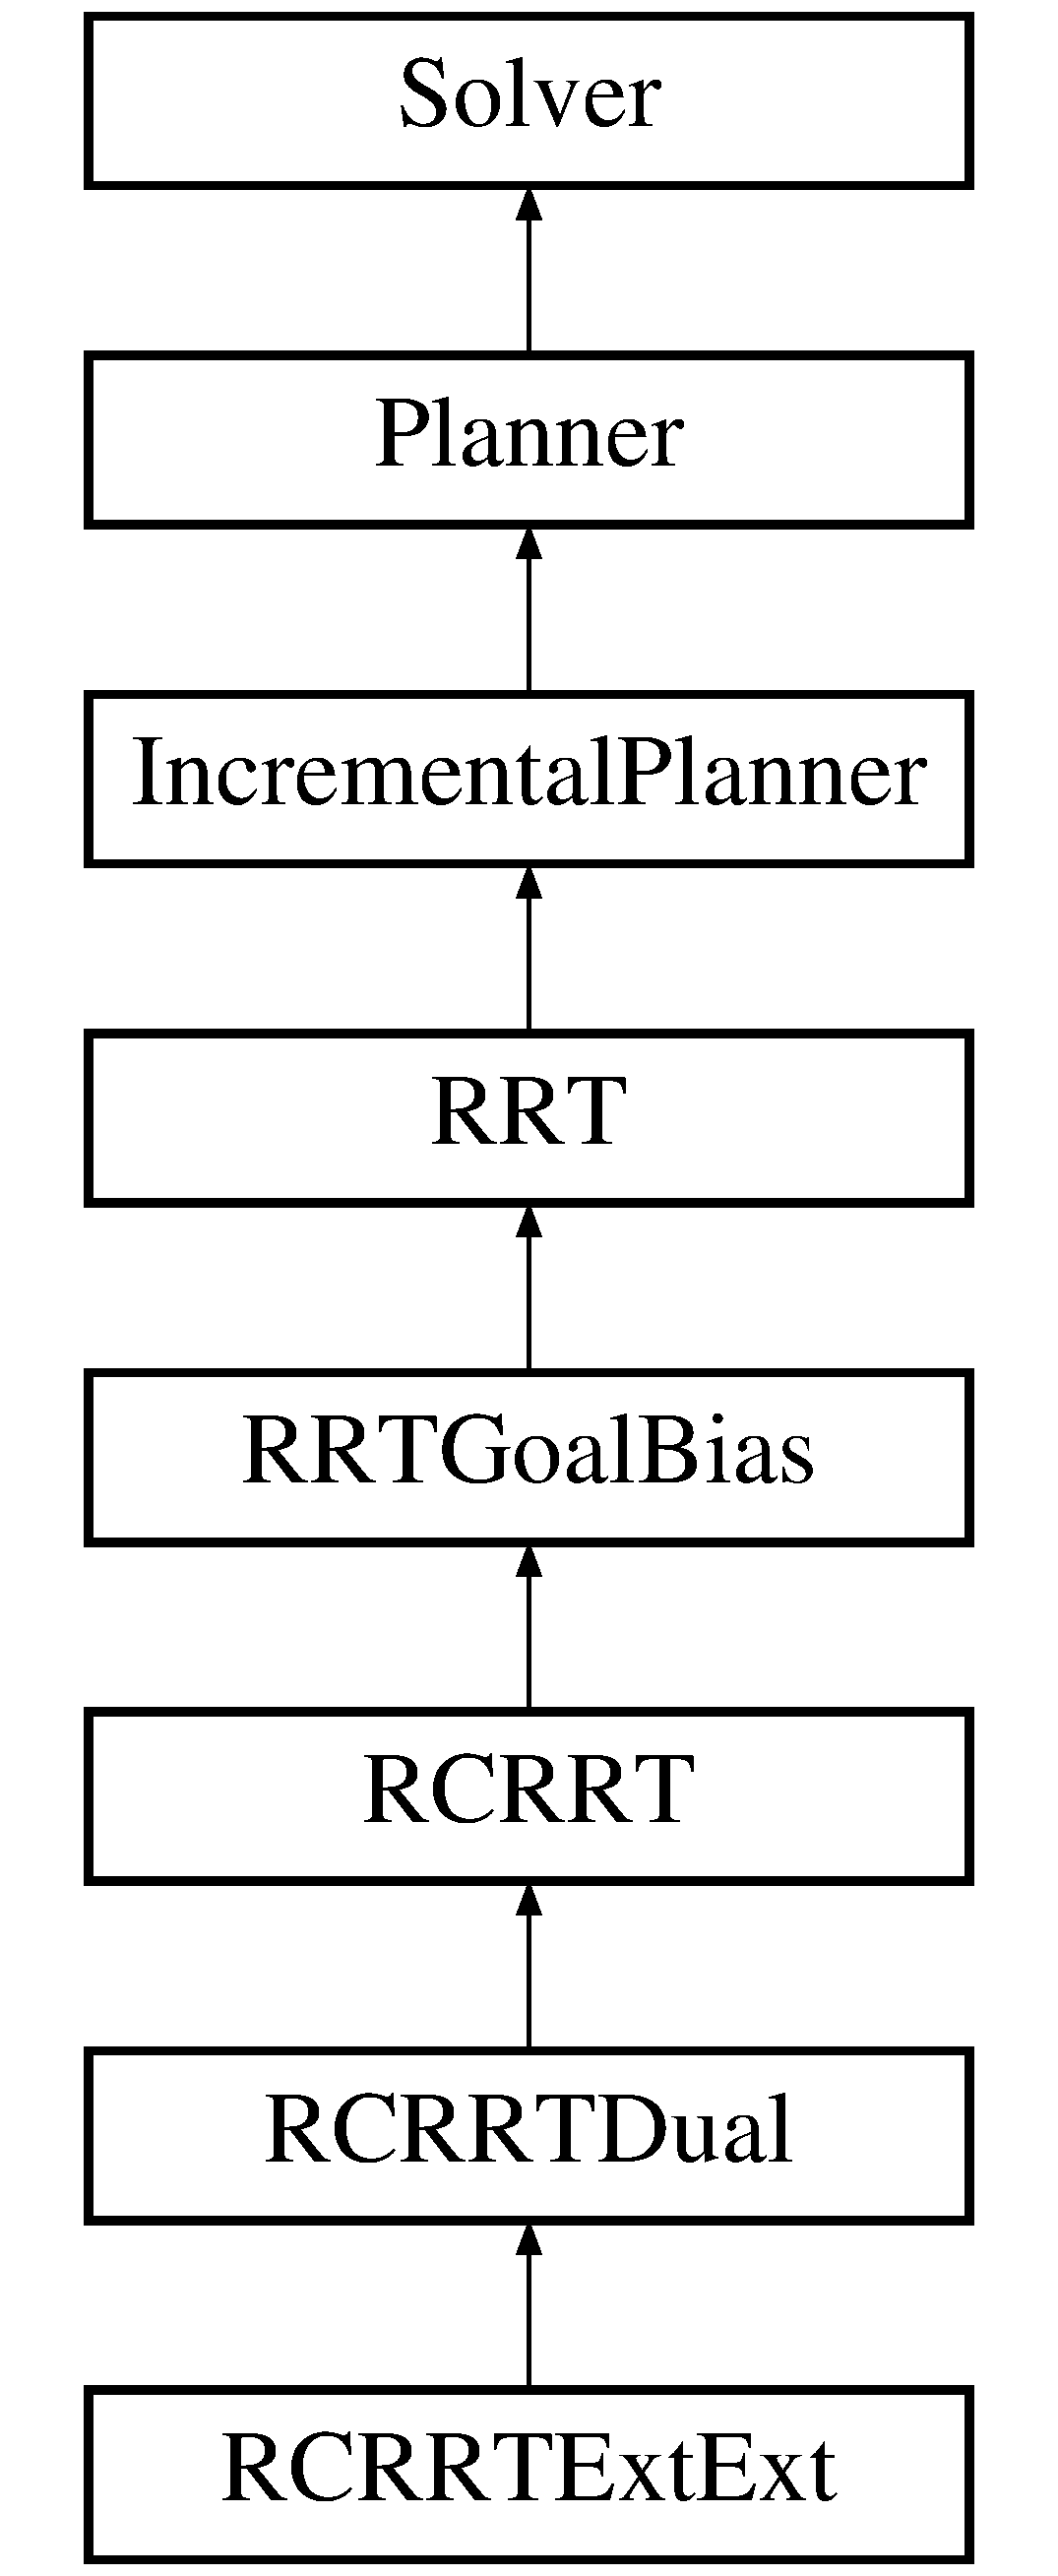
\includegraphics[height=8cm]{classRCRRTDual}
\end{center}
\end{figure}
\subsection*{Public Methods}
\begin{CompactItemize}
\item 
{\bf RCRRTDual} ({\bf Problem} $\ast$p)
\item 
virtual {\bf $\sim$RCRRTDual} ()
\item 
virtual bool {\bf Plan} ()
\begin{CompactList}\small\item\em Attempt to solve an Initial-Goal query by growing an {\bf RRT} {\rm (p.\,\pageref{classRRT})}.\item\end{CompactList}\item 
virtual bool {\bf Get\-Connected} ({\bf MSLNode} $\ast$n1, {\bf MSLNode} $\ast$n2)
\end{CompactItemize}
\subsection*{Protected Methods}
\begin{CompactItemize}
\item 
void {\bf Recover\-Solution} ({\bf MSLNode} $\ast$n1, {\bf MSLNode} $\ast$n2)
\end{CompactItemize}


\subsection{Detailed Description}
Basic dual tree version of {\bf RCRRT} {\rm (p.\,\pageref{classRCRRT})}.



\subsection{Constructor \& Destructor Documentation}
\index{RCRRTDual@{RCRRTDual}!RCRRTDual@{RCRRTDual}}
\index{RCRRTDual@{RCRRTDual}!RCRRTDual@{RCRRTDual}}
\subsubsection{\setlength{\rightskip}{0pt plus 5cm}RCRRTDual::RCRRTDual ({\bf Problem} $\ast$ {\em p})}\label{classRCRRTDual_a0}


\index{RCRRTDual@{RCRRTDual}!~RCRRTDual@{$\sim$RCRRTDual}}
\index{~RCRRTDual@{$\sim$RCRRTDual}!RCRRTDual@{RCRRTDual}}
\subsubsection{\setlength{\rightskip}{0pt plus 5cm}virtual RCRRTDual::$\sim$RCRRTDual ()\hspace{0.3cm}{\tt  [inline, virtual]}}\label{classRCRRTDual_a1}




\subsection{Member Function Documentation}
\index{RCRRTDual@{RCRRTDual}!GetConnected@{GetConnected}}
\index{GetConnected@{GetConnected}!RCRRTDual@{RCRRTDual}}
\subsubsection{\setlength{\rightskip}{0pt plus 5cm}bool RCRRTDual::Get\-Connected ({\bf MSLNode} $\ast$ {\em n1}, {\bf MSLNode} $\ast$ {\em n2})\hspace{0.3cm}{\tt  [virtual]}}\label{classRCRRTDual_a3}


\index{RCRRTDual@{RCRRTDual}!Plan@{Plan}}
\index{Plan@{Plan}!RCRRTDual@{RCRRTDual}}
\subsubsection{\setlength{\rightskip}{0pt plus 5cm}bool RCRRTDual::Plan ()\hspace{0.3cm}{\tt  [virtual]}}\label{classRCRRTDual_a2}


Attempt to solve an Initial-Goal query by growing an {\bf RRT} {\rm (p.\,\pageref{classRRT})}.



Reimplemented from {\bf RCRRT} {\rm (p.\,\pageref{classRCRRT_a10})}.

Reimplemented in {\bf RCRRTExt\-Ext} {\rm (p.\,\pageref{classRCRRTExtExt_a2})}.\index{RCRRTDual@{RCRRTDual}!RecoverSolution@{RecoverSolution}}
\index{RecoverSolution@{RecoverSolution}!RCRRTDual@{RCRRTDual}}
\subsubsection{\setlength{\rightskip}{0pt plus 5cm}void RCRRTDual::Recover\-Solution ({\bf MSLNode} $\ast$ {\em n1}, {\bf MSLNode} $\ast$ {\em n2})\hspace{0.3cm}{\tt  [protected]}}\label{classRCRRTDual_b0}




The documentation for this class was generated from the following files:\begin{CompactItemize}
\item 
{\bf rcrrt.h}\item 
{\bf rcrrt.C}\end{CompactItemize}
